\chapter{文献調査と問題提起}
\label{related_works}
\section{概要}
人間が使用する道具に機械や情報処理が介在し、高度で複雑なシステムになった現在、人間と道具との関係が問い直され、その関係をいかに設計するか、すなわちヒューマンインターフェースデザインが必要となった。そして、原始的な道具の使用感と同じように、原因と結果の対応が直接的であり、その道具を使っているという意識がなくなる「道具の透明化」こそが、その理想であるとされてきた\cite{Watanabe2017}。インターフェース研究者の渡邊は、その理想を実現する指針として「自己帰属感」という概念を導入し、例えばマウスカーソルやスマートフォンのような「操作時の指とグラフィックの追従性が高い」インターフェースは自身の一部や延長として感じられる、「透明」なインターフェースであると説明する。

確かにこうしたインターフェースを設計していくことは、複雑で高度な道具の力を借りて人間の活動の可能性を拡げることに貢献してきたが、人間と道具の関係とはそれだけだっただろうか?

コンピュータ工学研究者のSydney Felsは、オブジェクトと人との関係性を、「Embodiment」の観点から4つに分類した\cite{Fels}。
「Embodiment」については、認知科学やコンピュータ科学の理論用語にも同じ名前のものが存在する。中でも参照されることの多いものとして、認知科学者・哲学者である Gallagher\cite{Gallagher2000} の「ミニマルセルフ」という考え方が挙げられる。

Gallagheの論文が発表された2000年と同時期にこの分類を発表したFelsこの考えを参照していたのかはわからないが、Felsの捉えるEmbodimentは、「ミニマルセルフ」の説明とも重なる部分があり、相反する理論ではない。加えてFelsのEmbodimentにおいて特徴的なのは、人がオブジェクトを取り込み(Embody)、一体化することだけでなく、「オブジェクトが人を取り込む」という逆向きの一体化について論じていること、そして「一体化 (Embodiment) ではない状態」についても分類を行っていることである。

そこで本章ではまず、Gallagherの「ミニマルセルフ」とFelsによるEmbodimentを説明し、両者の関係について整理する。その上で、Felsの分類から改めて「技量の問題」による「使いにくさ」を説明し、それに着目した本研究が、Embodimentに着目している先行研究や作品と比べた上での、相違点について述べる。

\section{Gallagherのミニマルセルフ}
認知科学者・哲学者のGallagher\cite{Gallagher2000}は、自己を構成する2つの要素として、ミニマルセルフ(最小限の自己)とナラティヴ・セルフ(物語的自己)があると説明した。中でも「ミニマルセルフ」とは、一切の自己知識を失ったとしても残る最小限の自己であり、身体所有感(sense of ownership, body ownership)、行為主体感(sense of agency)の二つによって支えられていると説明する。

こうしたGallagherの分類に基づき、それらを評価する方法が考案され、ラバーハンド錯覚実験などにみられるように、生来の肉体ではないものを自分の身体と錯覚してしまうような、人間の身体像の曖昧さに注目した研究が認知科学や心理学の領域で取り組まれてきた。

こうした研究で蓄積された実証的知見は、インターフェースデザインや身体拡張の設計・評価へと応用されている。インターフェース研究者の渡邊は、機械や情報処理が介在する高度で複雑な道具であっても、「使っている最中にはその道具自体を意識せずに身体の一部になったかのようになり、目的に集中できる」こと、すなわち「道具の透明化」という、ヒューマンインターフェースの理想を実現するための指針としてこの概念に注目する。渡邊は、例えばマウスカーソルやスマートフォンのような「操作時の指とグラフィックの追従性が高い」インターフェースには「自己帰属感(Gallagherのsense of ownershipに対する訳語)」が生じるとし、このことからこうしたインターフェースは「自身の一部、延長」として考えられ、「道具の透明化」が実現すると説明する\cite{Watanabe2013}\cite{Watanabe2017}。

\section{FelsのEmbodiment}
一方でFelsは、オブジェクトと人との関係性について、Embodiment(身体化)が生じている状態について説明すると同時に、そうではない状態についても説明する、より広範な説明している。そうした関係性をFelsは、Reponse、Control、Gontemplation、Belongingの4つに分類した。それぞれの説明は以下の通りである。

\textbf{応答 Response:}\\
オブジェクトに対する働きかけの結果から、感情的な反応や理解を得る状態を指す。Felsはこの関係性の例として「コンピュータとそれに初めて触れた人」を挙げ、「なんらかの操作を通して得られた、便利な機能に喜んでいる状態、また逆に「有用な結果を得られず落胆する状態」と説明する。

\textbf{制御 Control:}\\
人がオブジェクトを自分自身の延長として使用し、その操作によって感情的な満足や美的体験を得る状態を指す。例えばピアノの演奏において、「音が出ている」ということだけでなく、自分自身の表現したいことが、不自由なくピアノを通して体現されていると感じるときの、一体感によってもたらされる心地よさがこれに該当する。

\textbf{鑑賞 Contemplation:}\\
人がオブジェクトに対して働きかけることはないが、人がそのオブジェクトからの信号やメッセージを内省や反映を通じて、感情的になったり美的体験を得る状態を指す。Felsはその具体例として、絵画の鑑賞体験を挙げる。

\textbf{帰属 Belonging:}\\
オブジェクトによって人が動かされているような経験を指す。人はそのオブジェクトによって提供される体験を通じて感情的な反応を得る。ここでは、オブジェクトが人の体験や感情を形作る役割を果たす。たとえばバイクの運転において、「バイクに合わせた走り方をする」といったように、単にそのオブジェクトを通して使い手の意図がそのまま体現されるのではなく、そのオブジェクトに合わせた振る舞いがそこで形作られることに喜びを見出すような状態である。

\begin{figure}[H]
  \centering
  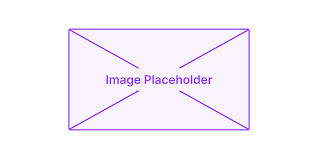
\includegraphics[width=15cm]{img/placeholder.png}
  \caption{FelsによるEmbodiment}
  \label{fig:fels_embodiment}
\end{figure}

さて、Felsは特に、上記「制御 Control」においては「自分自身の延長」として経験される感覚について言及しており、またそれが追従性の高いグラフィックによってもたらされるという記述は、渡邊がマウスカーソルやスマートフォンに対して用いた「操作時の指とグラフィックの追従性が高い」インターフェースという説明と同等のものである。このことからFelsのいうControlとは、Gallagherの「sense of ownership」と同じものを指していると考えられる。その上で、Embodimentの状態をControlのみならずBelongingから捉えていること、そしてEmbodimentが生じていない状態についても言及していることなど、現在HCIの分野で一般に用いられる意味でのEmbodimentよりも広く、人とオブジェクトを捉えるモデルとなっていることが確認できる。

さらにFelsは、オブジェクトと人とのあいだにある「深い関係」を指して、「Intimacy」という尺度で説明する。例えば楽器と人の関係性ように、Intimacyのある関係性のもとでは、「あたかもその装置が身体の延長であるかのように、考えや感情を効果的に表現できる」という。上記の、FelsによるEmbodimentの分類においては、ResponseがIntimacyの低い状態、ControlがIntimacyの高い状態として説明される。

ここまで見てきたように、

\section{身体性の変容に着目した研究}
親指の動きを肩の動きにマッピングさせる実験など、VRやロボティクスの分野でも取り組まれている研究では「sense of agency」や「sense of ownership」に基づく評価・設計が行われている。

\section{身体性の変容を扱った作品}
モデルトラッキングを用いて身体性の変容を扱った作品はいくつか存在する。小川らによる「えくす手(Metamorphosis Hand)」\cite{ekusute}では、指の伸びた手などの現実の身体にはあり得ない特性を持ったバーチャルな身体を通じてピアノを演奏することができる。そのねらいは、「現実とは異なる特性のバーチャルハンドへの身体所有感の生起を通じ、現実の身体的制約を超えたインタラクションを実現する、一種のバーチャルな身体拡張体験を提供する」と説明される。

身体所有感の生起要因に関するこれまでの議論を参照し、本作は「テクスチャ、形状、空間的配置、解剖学的構造の4つの特性」を根拠に、身体所有感が生じながらも、自己身体と意味的に類似しないバーチャルハンドを制作している。これらの特性は、身体所有感を生じさせる上での実証的知見ではあるが、本研究が対象とするIntimacyは、例えば楽器のように、こうした生起要因を押さえなくとも、習得を経て生じうるのではないかと考える。また、生起要因を多く踏襲しているわけではないからこそ、身体所有感が生じるまでには期間を必要とし、その程度にも個人差が生じるのではないだろうか。これらの観点から、本研究の取り組みは「えくす手」よりも極端な身体変容を促す体験として位置付けられる。

佐藤雅彦らによる「君の身体を変換してみよ展」はさまざまなアプローチで身体の変容を扱う作品が展示されたが、その中でも「点にんげん・線にんげん」という作品は、ボディトラッキングを用いて取得された全身の関節の位置を捉えたキーポイントが点として扱われ、異なる方法で結びつけられたり、ボロノイ分割が適用される点群として扱われるなど、さまざまな「変換」が行われている。\\
本作品との構造上の相違点として、関節の位置を捉えたキーポイントの並び替えの有無が挙げられる。佐藤らの作品では、身体の関節の位置を捉えたキーポイントはその配置を変えることなく、繋げ方やインターフェースの文脈における位置付けの違いで展開される。一方、本作ではキーポイントの配列もダイナミックに変化する。これは、手指が複雑な動きのできる器官であると同時に、身体の中でもっとも随意に動かすことのできる器官でもあることから、構造が大きく異なる場合でも、手指の動きに連動している箇所を、動かしている中で容易に同定できると考えているためである。


